\chapter{Visione artificiale}
\label{chap:visione}

\begin{minipage}{12cm}\textit{In questo capitolo verrà trattato il problema della generazione dei set di coppie di punti omologhi usando tecniche di visione. In particolare si utilizzeranno tecniche di Feature Detection e stereoscopia.}
\end{minipage}

\vspace*{1cm}

Nel capitolo \ref{chap:visualObs} si è accennato agli strumenti che sarebbero stati usati al fine della generazione dei suddetti set. In questo capitolo si procederà ad illustrarne il funzionamento con maggior dettaglio e si fornirà una possibile soluzione al problema. Conviene definire per primo il problema che si vuole affrontare.

\begin{prob}
	\label{prob:vis:gensets}
	Sia un osservatore mobile dotato di almeno due fotocamere. Si supponga ancora capace di "catturare", attraverso le suddette fotocamere, coppie di foto in diversi istanti (anche regolari). Allora: 
	\begin{enumerate}
		\item è possibile, utilizzando le informazioni fornite dalle fotocamere, calcolare le coordinate spaziali (in $\mathbb{R}^3$) di un punto del mondo (o più di uno) nel sistema di riferimento solidale all'osservatore?
		\item dato un punto del mondo (o più di uno) per il quale si è riusciti a calcolarne le coordinate spaziali, è possibile individuare lo stesso punto, in un altro istante del tempo, se l'osservatore si è mosso e se lo stesso è ancora visibile?  
	\end{enumerate}
\end{prob}

\section{Feature Detection e Matching}
\label{sec:feature}
Per \textbf{Feature Detection} o \textbf{individuazione dei punti chiave} in italiano, si intende un particolare settore facente parte della branca della visione artificiale, il cui scopo è quello di per l'appunto l'individuazione, la descrizione e il confronto delle Feature. Ma che cosa è una Feature?
In generale risulta difficile fornire una definizione chiara di cosa è una \textbf{Feature} o \textbf{Punto chiave}, può dipendere ad esempio dall'algoritmo che si utilizza o da scelte implementative.


\begin{figure}[h]
	\centering
	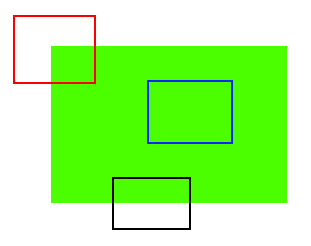
\includegraphics[width=420pt]{imgs/feature_simple.png}
	\caption{Individuazione delle Features.}
	\label{vis:feature:detect}
\end{figure} 

Si faccia ad esempio riferimento alla figura \ref{vis:feature:detect}, si supponga di dover individuare una buon punto chiave, il quale possa essere facilmente riconosciuto e riposizionato. Si consideri per prima la porzione di immagine evidenziata dal riquadro blu; è chiaro che qualora si dovesse scegliere dove posizionare tale blocco, si avrebbero un numero elevatissimo di possibilità ed in nessun caso si potrebbe avere al certezza di un buon posizionamento. Si consideri allora il blocco nero, in questo caso il numero delle possibilità è sicuramente inferiore, infatti esso può essere posizionato solo nel lato inferiore del rettangolo verde in figura. Infine si consideri il blocco rosso, è chiaro che quello in figura è l'unico punto in cui esso può essere posizionato.
L'esempio precedente fornisce un importantissimo spunto ri riflessione su cosa può essere una Feature e cosa no. Infatti sicuramente una porzione di immagine uniforme non può essere un punto chiave; se invece si considerano dei contorni di un oggetto la situazione migliora. In particolare se si considera il contorno di un oggetto e se ne sceglie un punto che abbia una forma o pattern particolare, come ad esempio uno spigolo di un oggetto, risulta molto più facile un eventuale riconoscimento. 

Ovviamente l'esempio precedente risulta estremizzato. Infatti, in un caso reale, le Feature possono essere ruotate e/o scalate e questo complica il problema. Al contempo però, il mondo reale risulta più dettagliato e risulta più difficile avere uno stesso pattern in punti diversi.

Si è fornita, quanto meno in modo informale, una definizione di Feature. Nei prossimi paragrafi con ordine si illustreranno tre algoritmi: il primo adibito all'individuazione delle features, il secondo viene impiegato per la generazione dei descrittori (che come si vedrà sono utilizzati per distinguere i punti chiave in base alle informazioni fornite dall'immagine) ed il terzo è sostanzialmente un matcher. 

%\subsection{Definizioni e problema}
%\label{sec:det:def}


\subsection{L'algoritmo FAST}
\label{sec:det:fast}

\subsection{L'algoritmo BRIEF}
\label{sec:det:brief}

\subsection{Brute Force matching}
\label{sec:det:bmmatch}


\section{Stereoscopia}
\label{sec:stereo}


%\subsection{Definizioni e problema}
%\label{sec:stereo:def}


\subsection{Modello matematico del sensore fotografico}
\label{sec:stereo:modello}


\subsection{Ricostruzione 3D}
\label{sec:stereo:ric3d}


\section{Soluzione al problema}
\label{sec:vision:solution}


